\section{Illumination globale}

\begin{frame}{Eclairage direct versus indirect}
    \begin{columns}
        \begin{column}{0.49\textwidth}
            \begin{center}
                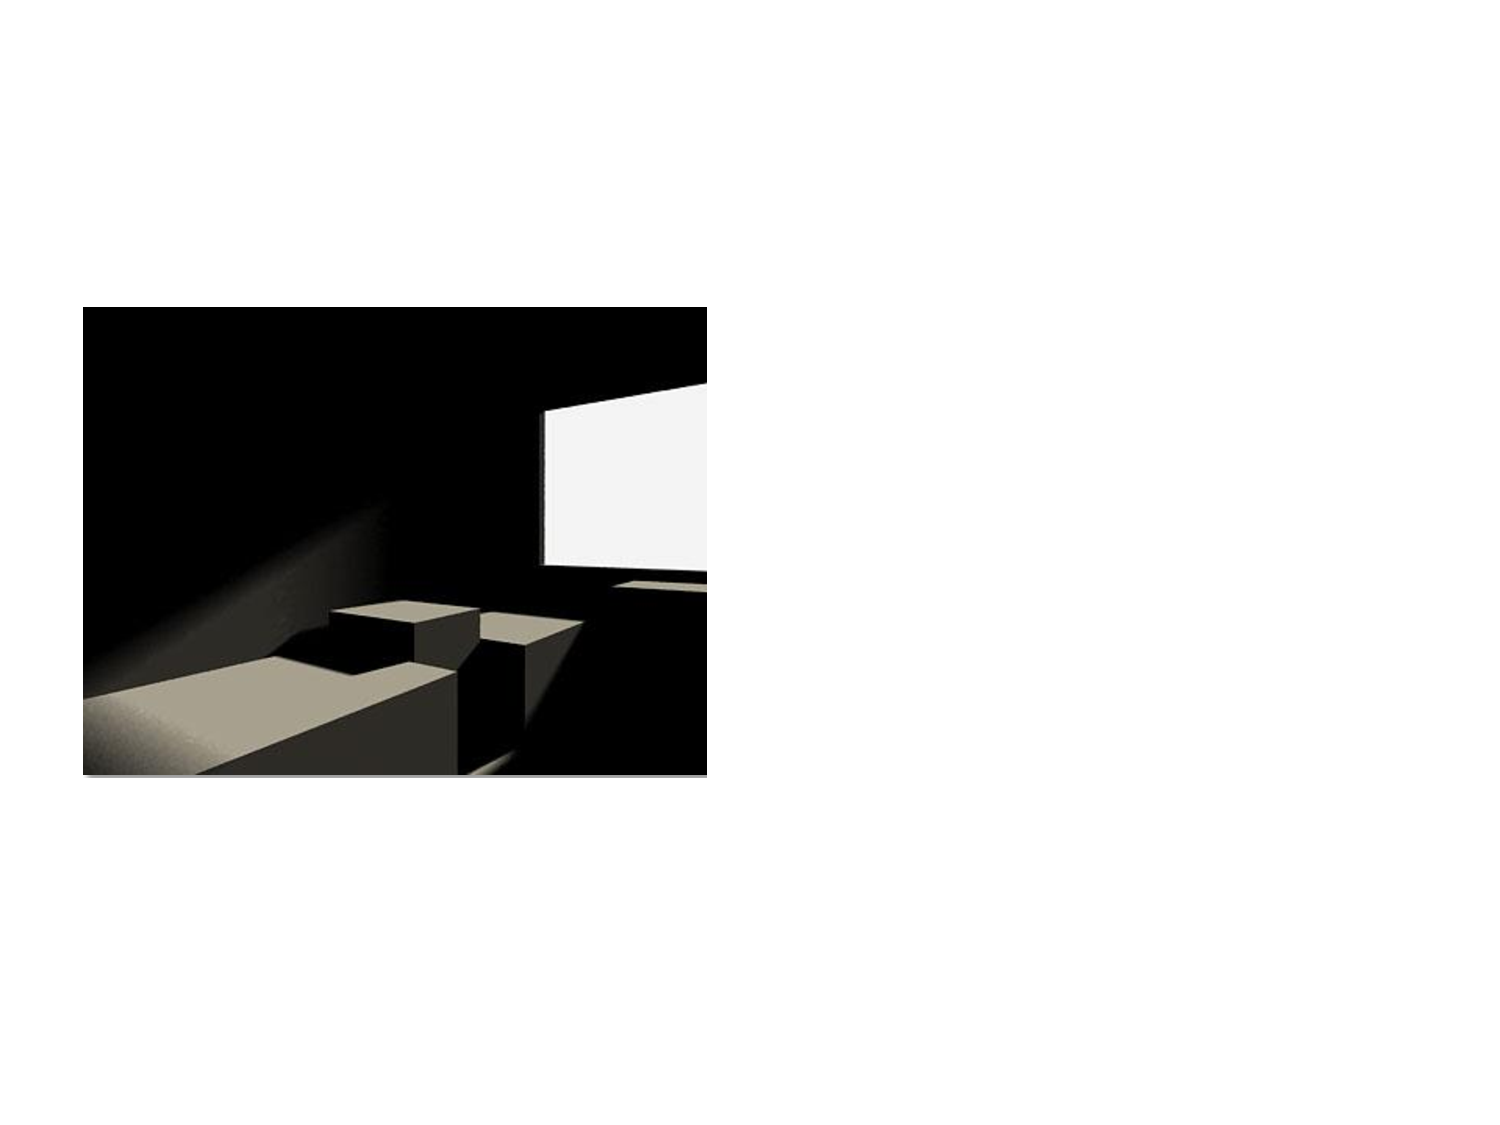
\includegraphics[width=\columnwidth]{figs/eclairage-direct.pdf}
                Eclairage direct : propriétés locales 
            \end{center}
        \end{column}
        \begin{column}{0.49\textwidth}
            \begin{center}
                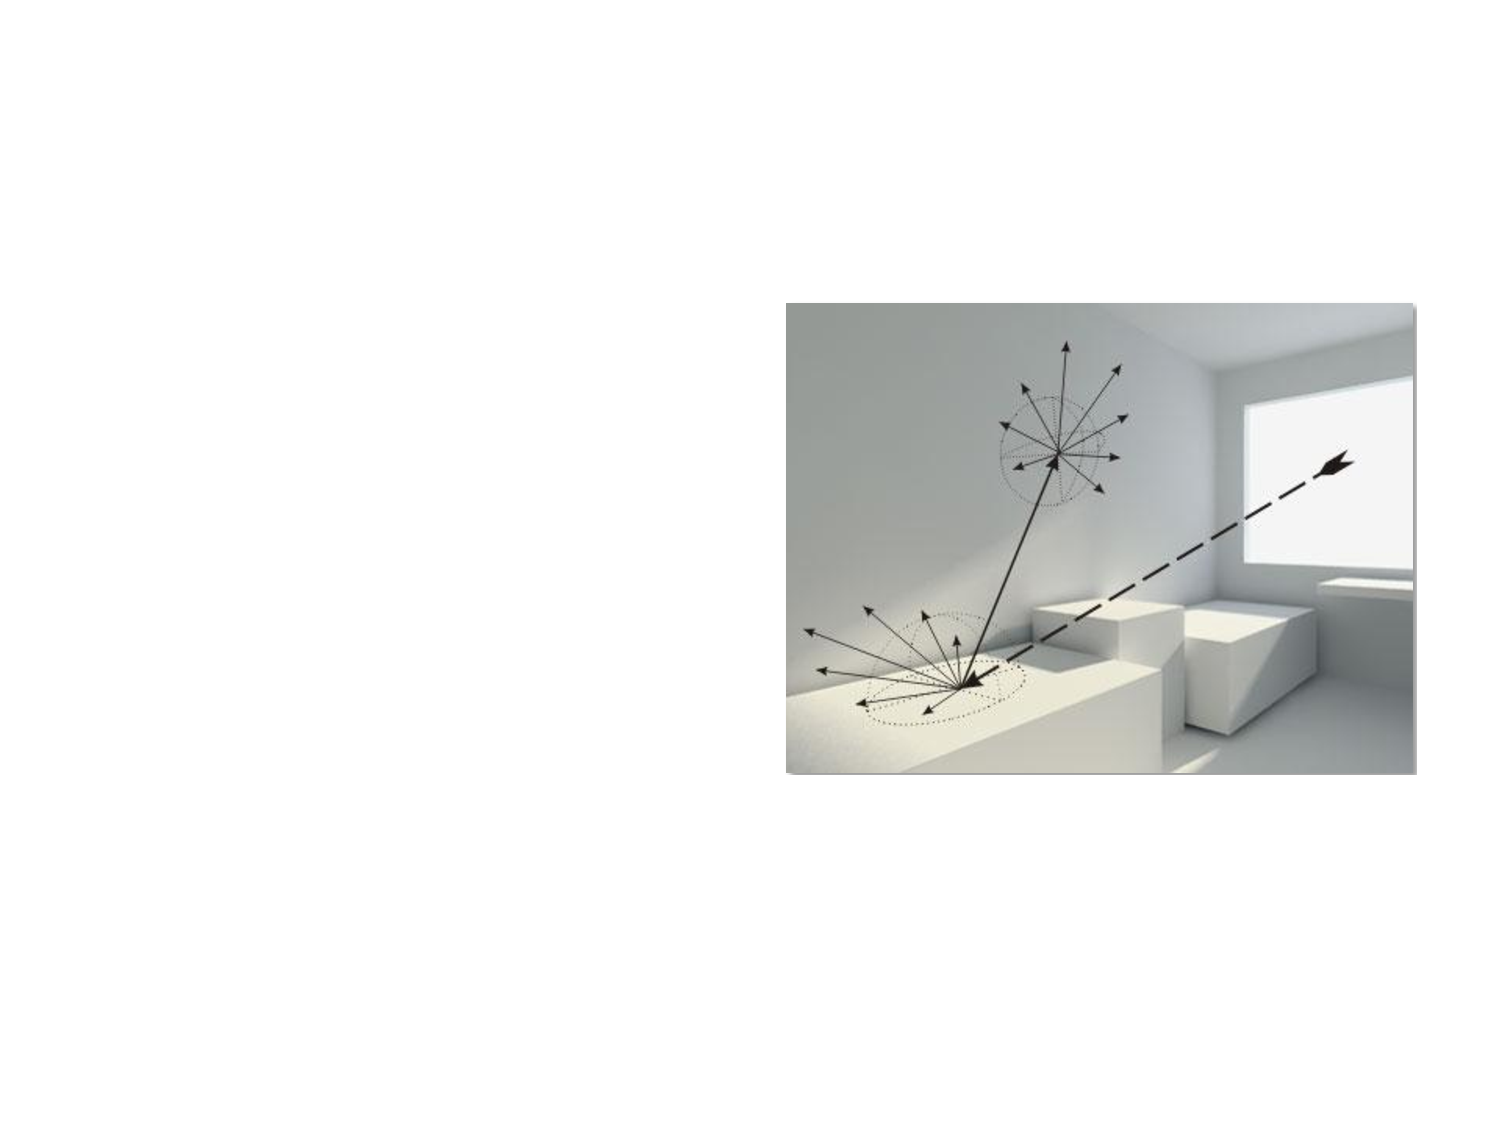
\includegraphics[width=\columnwidth]{figs/eclairage-indirect.pdf}
                Eclairage indirect : problème global
            \end{center}
        \end{column}
    \end{columns}
\end{frame}

\begin{frame}{Eclairage global versus local}
\begin{itemize}
    \item Jusqu'ici des propriétés locales 
    \begin{itemize}
        \item Modèle de Gouraud, de Phong, lissage 
        \item Placage de textures 
    \end{itemize}
    \item Algorithmes locaux
    \begin{itemize}
        \item Z-buffer, Peintre
    \end{itemize}
    \item Très (très) rapide 
\end{itemize}    
\end{frame}

\begin{frame}{Résultat}
    \begin{columns}
        \begin{column}{0.49\textwidth}
            \begin{center}
                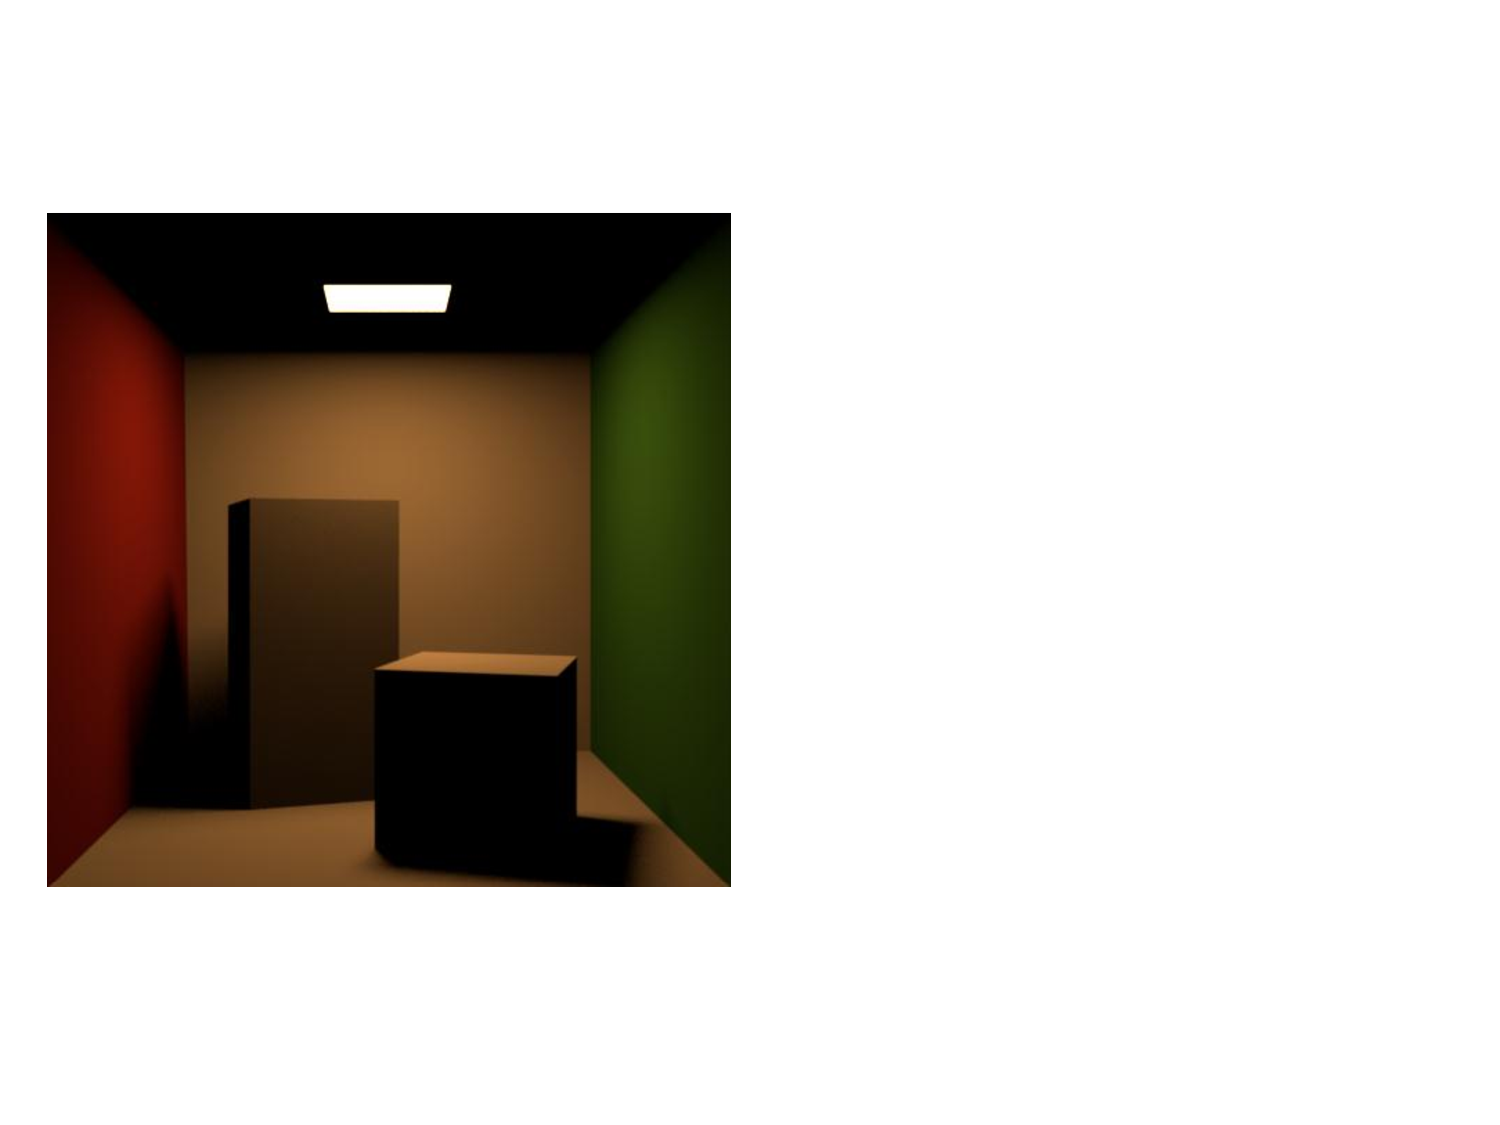
\includegraphics[width=\columnwidth]{figs/rendu-direct.pdf}
                Eclairage direct 
            \end{center}
        \end{column}
        \begin{column}{0.49\textwidth}
            \begin{center}
                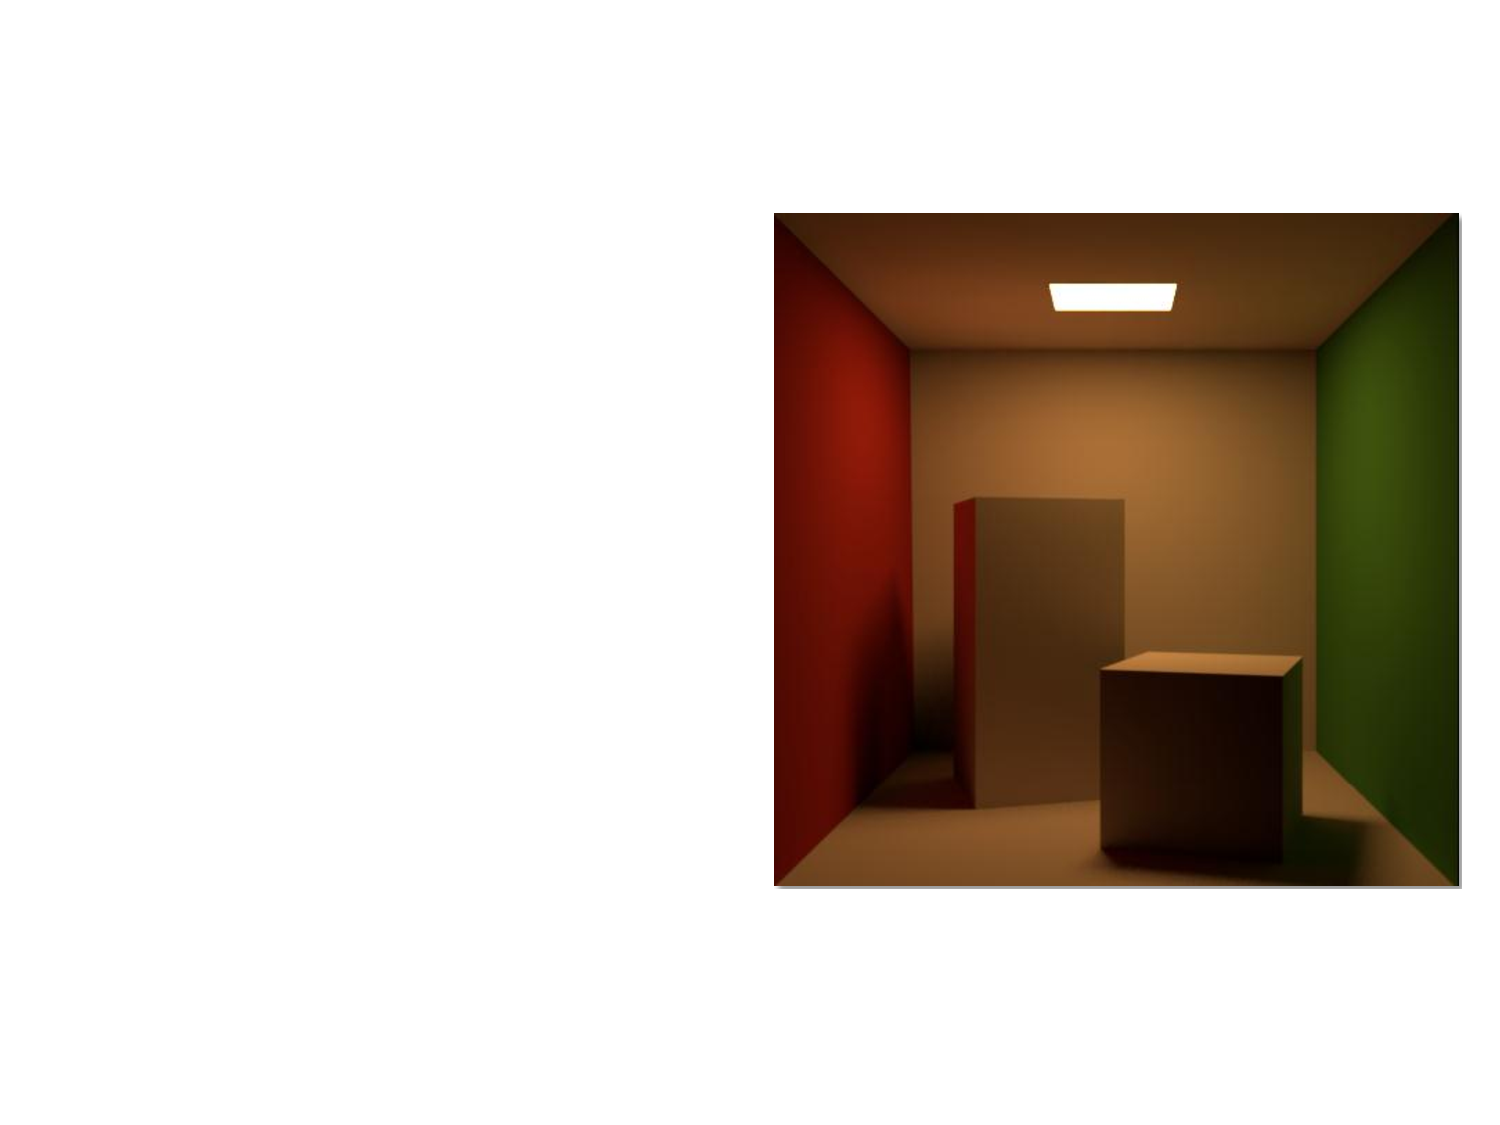
\includegraphics[width=\columnwidth]{figs/rendu-indirect.pdf}
                Eclairage indirect 
            \end{center}
        \end{column}
    \end{columns}
\end{frame}

\begin{frame}{Motivation}
    \begin{center}
        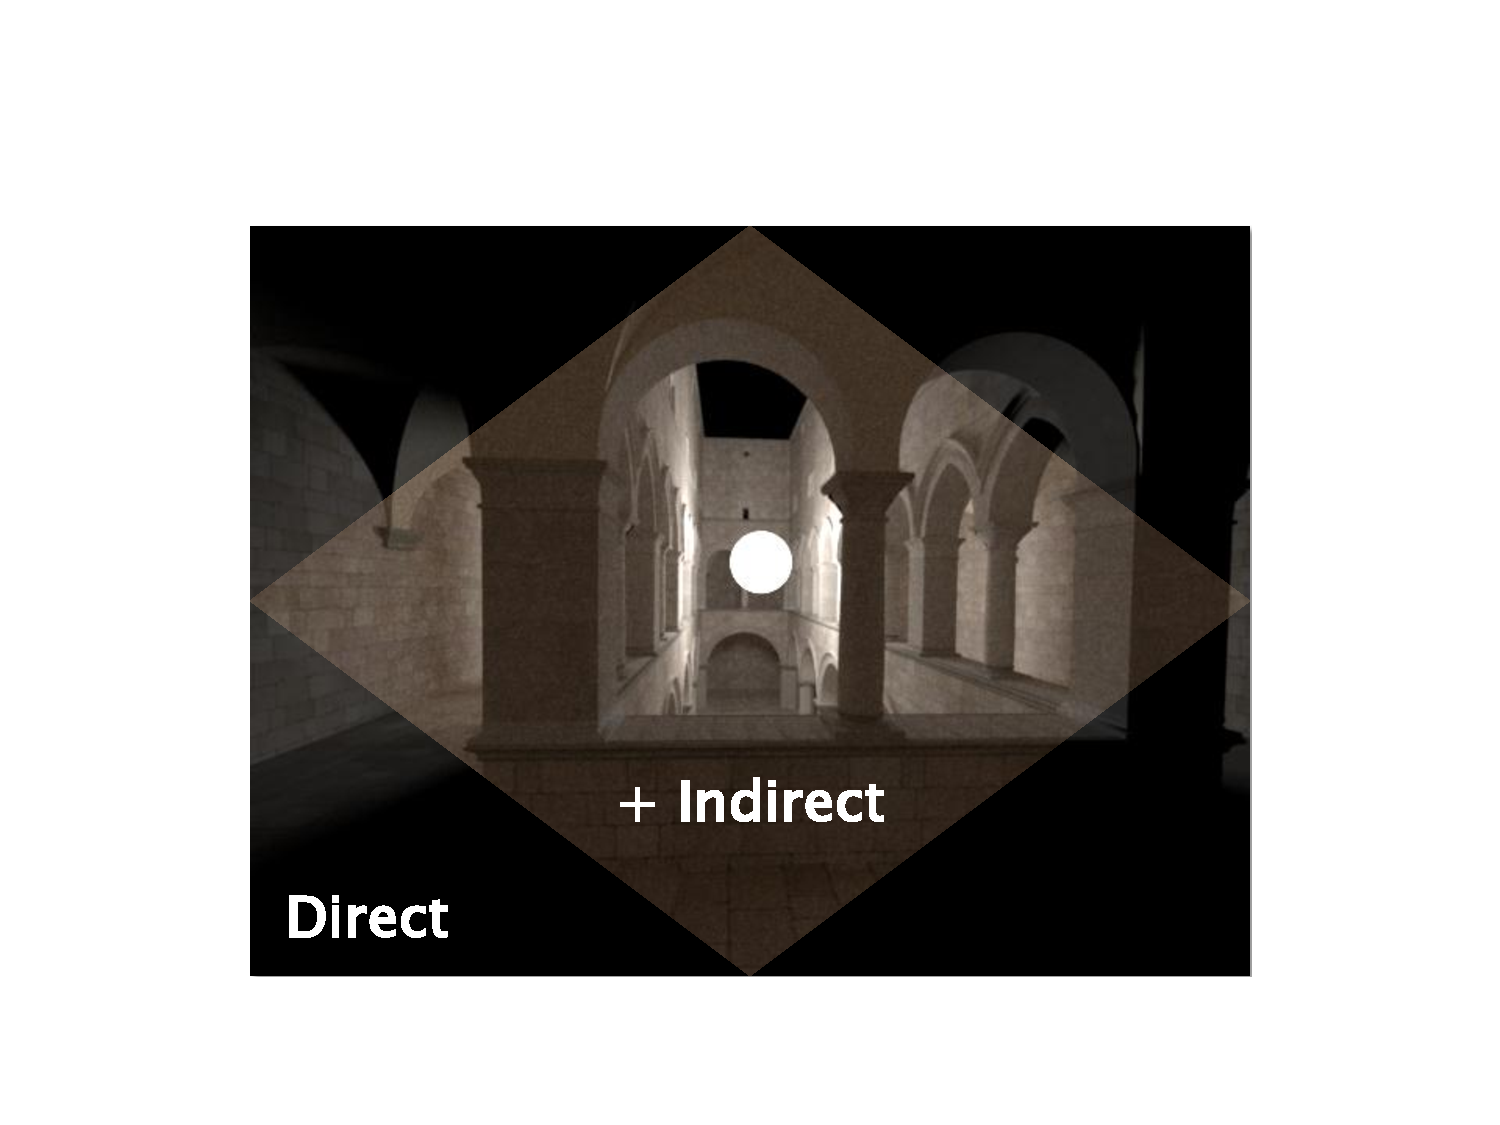
\includegraphics[width=.7\textwidth]{figs/motivation.pdf}
    \end{center}
\end{frame}

\begin{frame}{Illumination globale}
\begin{itemize}
    \item Interactions entre objets 
    \item Transport de la lumière 
    \item Réflexions, réfraction, diffusion
    \item Conservation de l'énergie lumineuse 
\end{itemize}
\begin{center}
    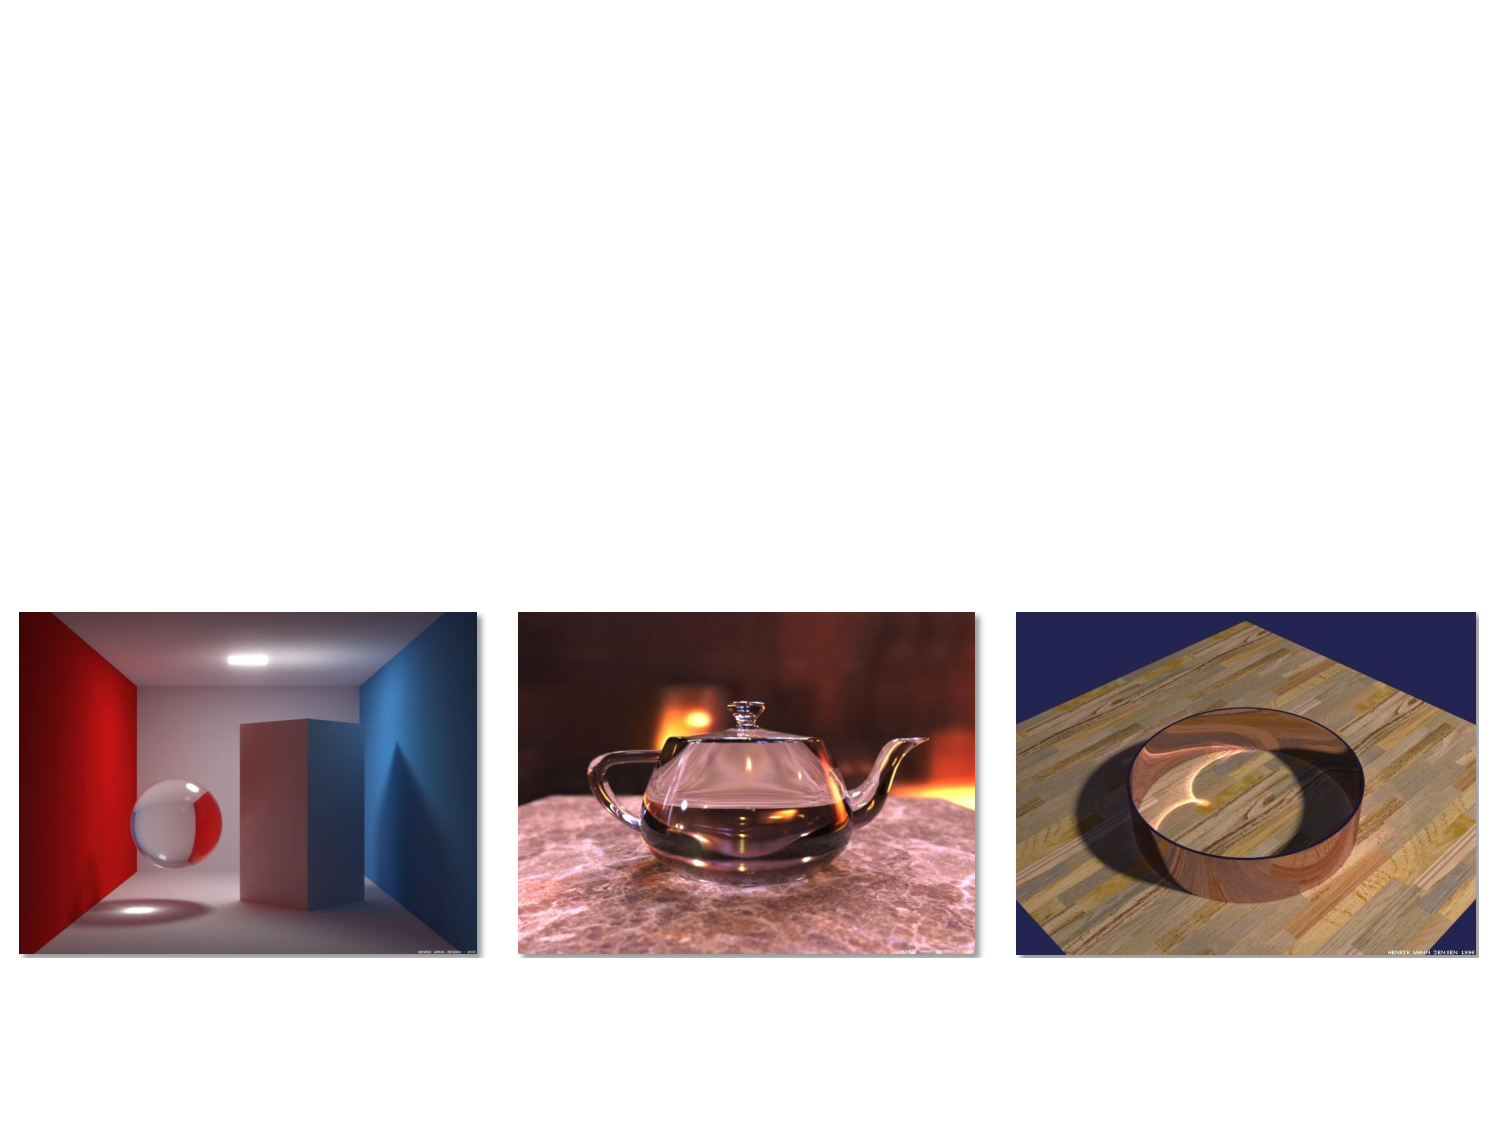
\includegraphics[width=\textwidth]{figs/illumination-globale.pdf}
\end{center}
\end{frame}

\begin{frame}{Equation de l'éclairage}
    \begin{itemize}
        \item Hypothèses 
        \begin{itemize}
            \item Equilibre énergétique 
            \item Conservation de l'énergie ... lumineuse 
            \item i.e. pas d'échanges entre différents types d'énergie 
        \end{itemize}
        \item Energie lumineuse (radiance) en un point (petite unité de surface)
        \item \begin{itemize}
            \item Energie émise (source de lumière)
            \item + énergie réfléchie depuis les autres surfaces
        \end{itemize}
    \end{itemize}
\end{frame}

\begin{frame}{Equation de l'éclairage}
\begin{center}
    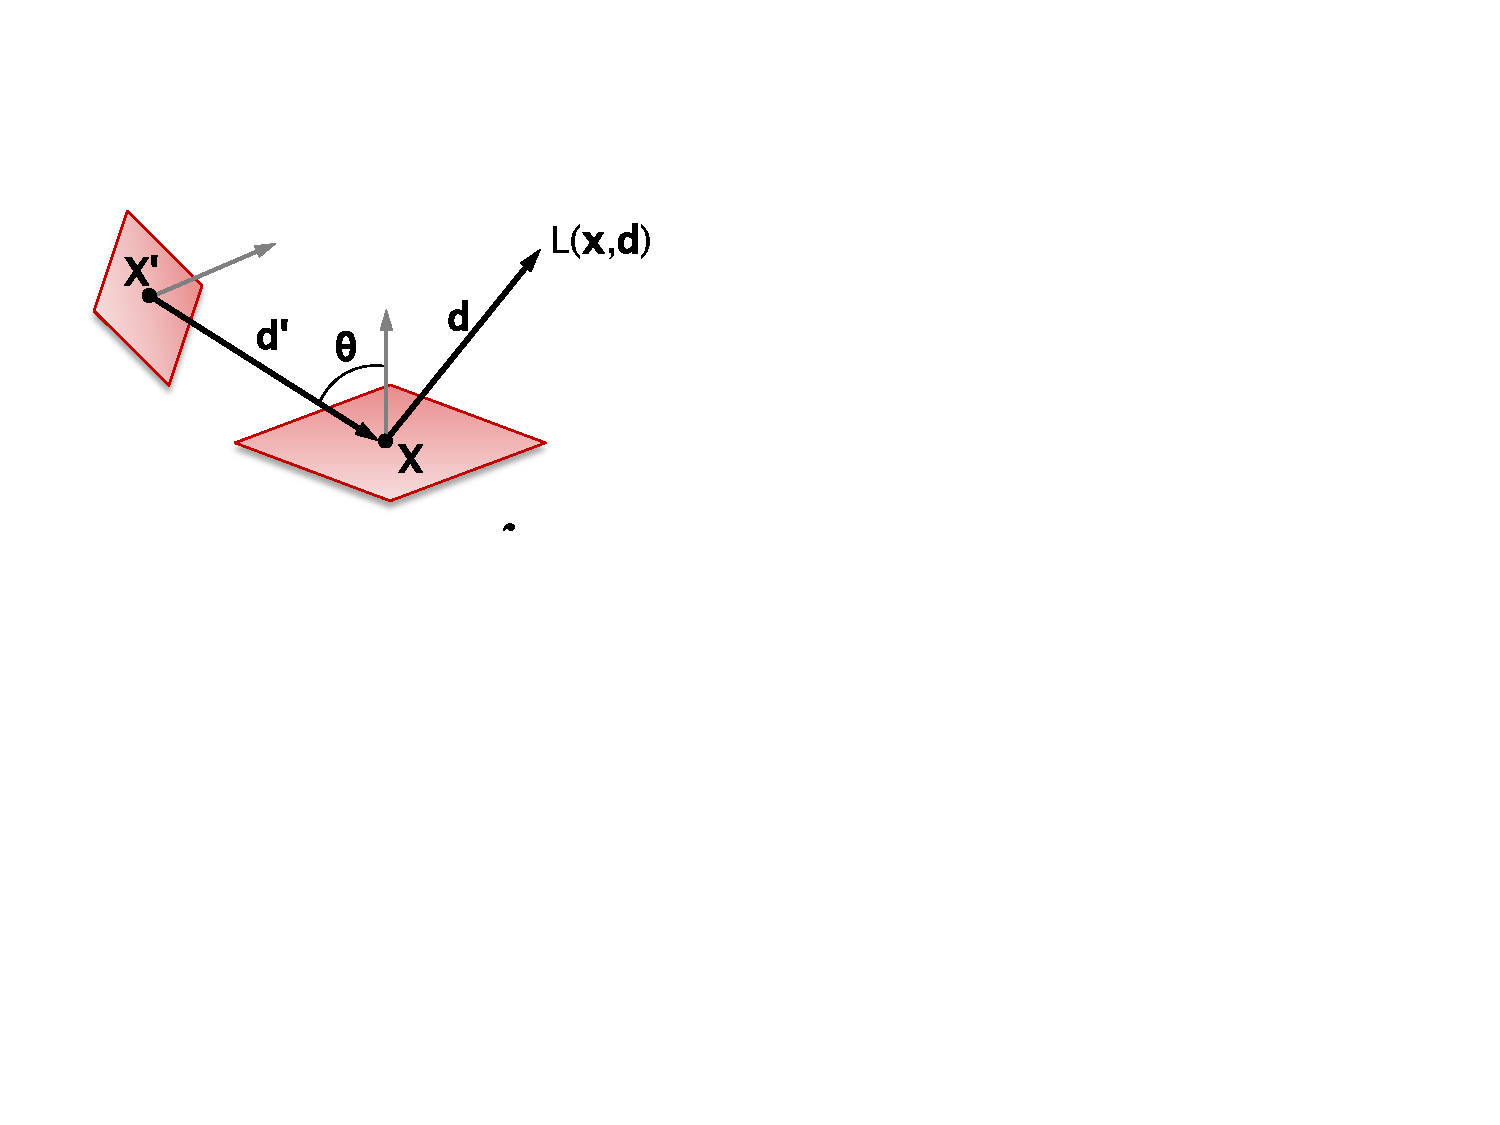
\includegraphics[width=.5\textwidth]{figs/eq-eclairage.pdf}
\end{center}

    $$
    L(x,d) = E(x,d) + \int \rho(x,d,d')v(x,x')L(x',d')G(x,x')  \,\mathrm{d}A 
    $$

\end{frame}


\begin{frame}{Equation de l'éclairage}
    $$
    L(x,d) = E(x,d) + \int \rho(x,d,d')v(x,x')L(x',d')G(x,x')  \,\mathrm{d}A 
    $$
avec :
\begin{itemize}
    \item $L(x,d)$ : radiance sortante en un point $x$ dans la direction $d$ 
    \item $E'x,d)$ : radiance émise par le point $x$, non nulle uniquement pour les sources de lumière
    \item $\int \rho(x,d,d')v(x,x')L(x',d')G(x,x')  \,\mathrm{d}A$ : intégration des contributions de toutes les surfaces, dont
    \begin{itemize}
        \item $L(x',d')$ : radiance incidente depuis $x'$ dans la direction $d'$
        \item $\rho(x,d,d')$ : réflectance (BRDF) de la surface en $x$ 
        \item $v(x,x')$ : visibilité entre $x$ et $x'$ : 0 ou 1 
        \item $G(x,x')$ : description de la relation géométrique entre les deux surfaces en $x$ et $x'$
    \end{itemize}
\end{itemize}
\end{frame}

\begin{frame}{Equation de l'éclairage : solutions}
\begin{block}{Problème}
    Solution analytique générale impossible !
\end{block}
\begin{itemize}
    \item 2 grandes familles de solutions approchées
    \item Version (très) simplifiée
    \item Radiosité 
    \begin{itemize}
        \item tous les objets sont diffus 
    \end{itemize}
    \item Lancer de rayons 
    \begin{itemize}
        \item tous les objets sont spéculaires 
    \end{itemize}
\end{itemize}
\end{frame}

\subsection{Lancer de rayons}

\begin{frame}{Le lancer de rayons}
    \begin{center}
        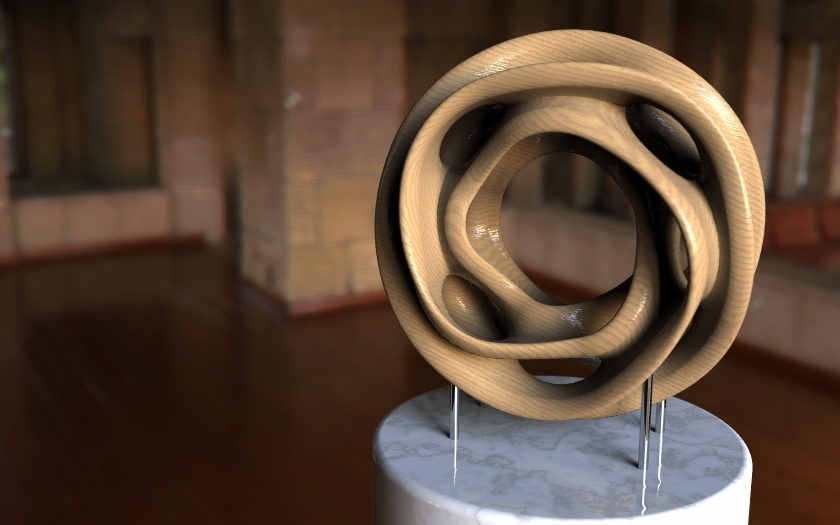
\includegraphics[width=.4\textwidth]{figs/sherk-collins.jpg}\\
        {\tiny "Scherk-Collins sculpture" by Trevor G. Quayle (2008)}
    \end{center}
    \begin{itemize}
        \item Algorithme : Appel, 1968 
        \item Logiciel : Goldstein et Nagel, 1971
        \item Exemple célèbre (et gratuit) : povray, \url{http://www.povray.org}
        \item Idée générale
        \begin{itemize}
            \item Chaque facette est un réflecteur parfait 
            \item Inverser la circulation des rayons lumineux : de l'écran vers les sources de lumière
        \end{itemize}
    \end{itemize}
\end{frame}

\begin{frame}{Inverser le chemin des rayons lumineux}
    \begin{center}
        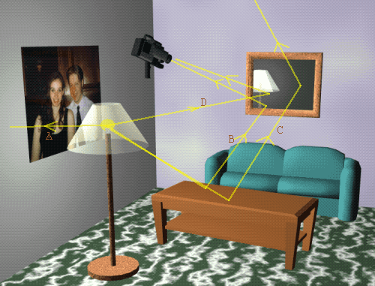
\includegraphics[width=.6\textwidth]{figs/rt-inverse.png}
    \end{center}
    Pourquoi ? 
    L'écran a un nombre fini de pixels, on va lancer un rayon de chaque pixel
\end{frame}

\begin{frame}{Principe}
    \begin{columns}
        \begin{column}{.49\textwidth}
            \begin{itemize}
                \item Pour chaque pixel, on calcule la demi-droite ayant pour origine un pixel du plan image de la caméra et passant par son centre optique 
                \item On cherche ensuite l'intersection entre cette demi-droite et un élément de la scène puis on utilise un modèle d'illumination local
                \item S'il n'y en a pas, le point sera noir
            \end{itemize}
        \end{column}

        \begin{column}{.49\textwidth}
            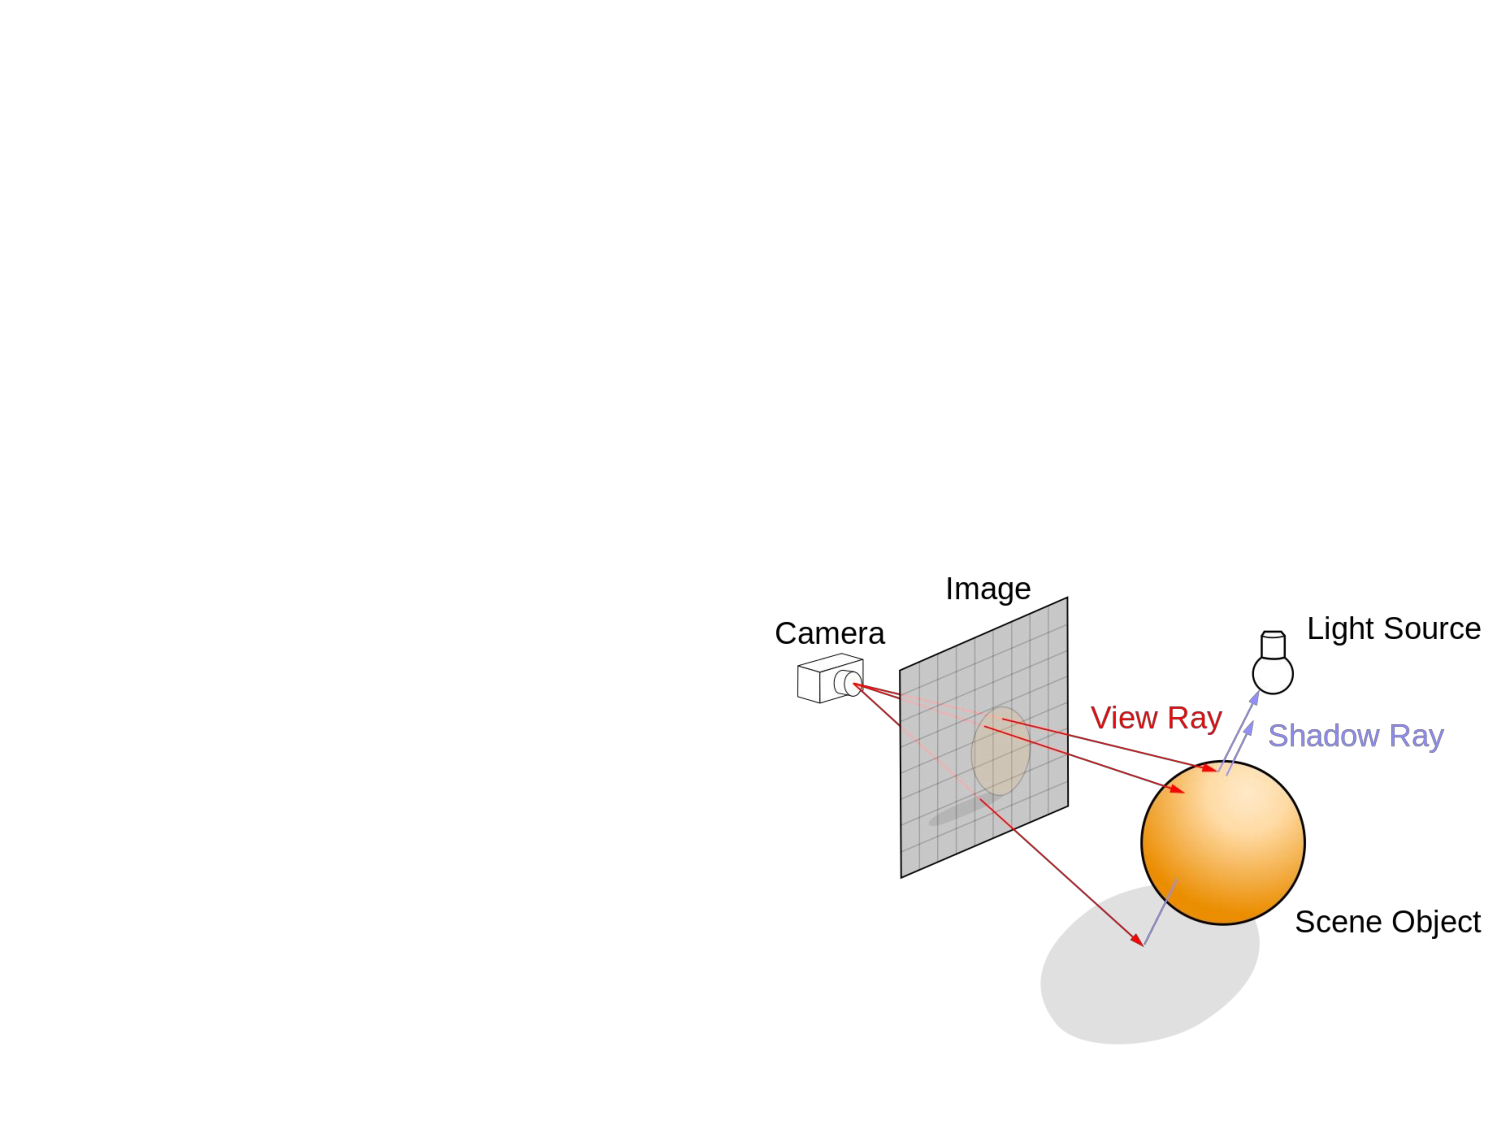
\includegraphics[width=\columnwidth]{figs/raycasting.pdf}
        \end{column}
    \end{columns}
\end{frame}

\begin{frame}{Lancer de rayons selon Whitted}
    \begin{itemize}
        \item Whitted a proposé d'ajouter à cela les lois de la diffraction / réfraction et les réflexions à chaque fois qu'un rayon rencontre un objet de la scène
        \item Cela donne un algorithme récursif : un rayon qui rencontre un objet génère deux autres rayons
        \begin{itemize}
            \item Un rayon réfléchi 
            \item Un rayon transmis
        \end{itemize}
    \end{itemize}
\end{frame}

\begin{frame}{Réflexion}
    \begin{center}
        \animategraphics[loop,controls,width=.5\linewidth]{10}{figs/rt-reflection/}{0}{8}
    \end{center}
\end{frame}

\begin{frame}{Réfraction}
    \begin{center}
        \animategraphics[loop,controls,width=.5\linewidth]{10}{figs/rt-refraction/}{0}{8}
    \end{center}
\end{frame}
